\section{Objectifs du projet}

L'objectif de ce projet est de concevoir et de développer un interpréteur de L-système qui prendra en entrée des règles de réécriture et produira une représentation visuelle en 2D (ou éventuellement en 3D) de l'objet généré par la simulation du système. Pour cela, plusieurs étapes devront être réalisées, notamment la conception d'un parser pour analyser les règles de réécriture, la mise en place d'un moteur de réécriture pour appliquer les règles successivement, et enfin la mise en œuvre d'un moteur de rendu graphique pour visualiser le résultat final.

Le projet pourra être étendu pour prendre en compte les L-systèmes stochastiques, où les règles sont appliquées avec une probabilité donnée, ainsi que les L-systèmes contextuels, où les règles sont appliquées en fonction des symboles environnants. La réalisation de cet interpréteur de L-système permettra ainsi de créer des modèles végétaux réalistes et diversifiés, offrant de nombreuses possibilités pour les applications dans le domaine du jeu vidéo, de l'animation et de la modélisation graphique.


\subsection{Description des grandes étapes et fonctionnalités à implémenter}

\subsubsection{Partie 0 : réalisation de la version 1 diagramme UML}
LA Figure 1 représente le tous premier diagramme UML réaliser par notre groupe  , il a été modifier réguliarement.
\begin{figure}[h]
\centering
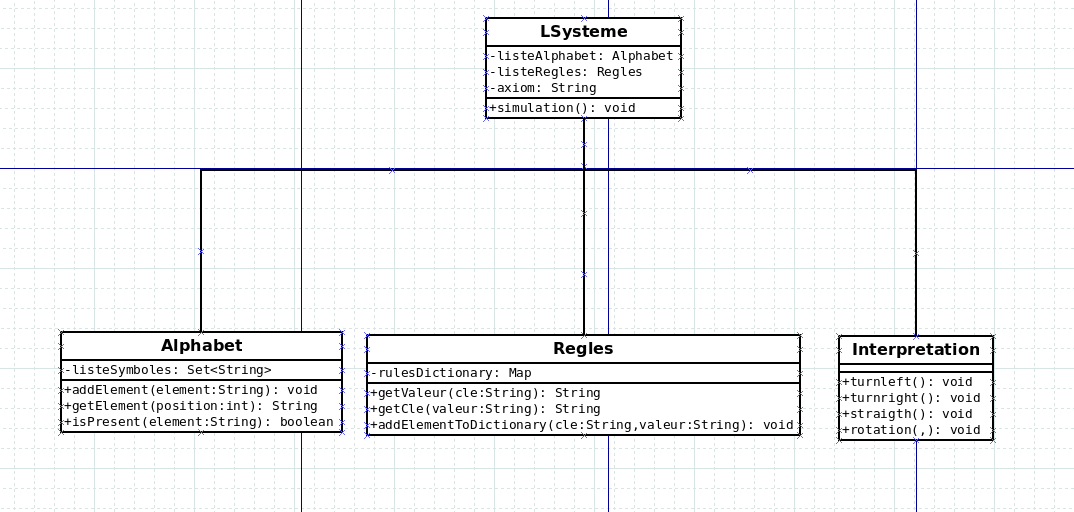
\includegraphics[scale=0.3]{images/version1UML.png}
\caption{Premier diagramme UML réaliser}
\end{figure}
\subsubsection{Partie 1: Définition d'un langage pour construire un système de Lindenmeyer classique}

\begin{enumerate}
    \item Description de la syntaxe et de la grammaire du langage utilisé pour représenter les règles de réécriture d'un L-système.Exemple \textbf{A,B,C......Z} , \textbf{+,-,*,/,[,]};
    \item   Présentation des éléments de base d'un L-système, tels que les symboles, les règles de réécriture, les axiomes et les paramètres.
    \item Ecrire les contrats de chaque fonction avant l'implémentation .
    \item  \label{hash} Implémentation d'un parser pour analyser les règles de réécriture d'un L-système en entrée et les représenter dans une structure de données adaptée dans le code .Le parser utilisé dans notre code est le \textbf{HashMap}(dictionnaire ), exemple de régle avec \textbf{HashMap}:\\
    
\begin{center}
    \fbox{
   
    \begin{minipage}{0.4\textwidth}
    \centering
       \{ \\
            "A": "AB",\\
            "B": "A"\\
        \} \\
    \end{minipage}
}
\end{center}
   
\end{enumerate}
    
   

\subsubsection{Partie 2: Implémentation d'un interpréteur pour une visualisation 2D}

\begin{enumerate}
   
    \item  Explication du processus de réécriture itératif qui génère une séquence de symboles à partir de l'axiome initial en appliquant les règles de réécriture successivement.\\
     \fbox{
   
        \begin{minipage}{0.9\textwidth}
        
            Le moteur représente la fonction "simulation(....)" dans notre code ,tels que cette  fonction  est une fonction hypothétique déclarer dans le package model/classe AbstractLsystem . Cette fonction représente le moteur de réécriture d'un L-système, qui prend en entrée un axiome initial (souvent sous forme de chaîne de caractères OU meme  caractére), les règles de réécriture définies pour ce L-système la liste \textbf{HashMap}, ainsi que le nombre d'itérations souhaitées pour appliquer ces règles.
          \end{minipage}
    }
    \item   Interprétation des symboles générés comme des instructions de dessin pour tracer la structure arborescente sur un canvas 2D.En utilisant la fonction "rotation2D(....)" .
    \item  Présentation d'exemples de structures végétales générées à partir du L-système en utilisant des fichiers \textbf{.txt} contenant les coordonnées des points [ x y ] a dessiner sachant que les points sont calculer generer a partir des fonctions implémenter dans model comme "calculCoordinate(...)" puis copier
    apartir du terminal et coller dans differents fichiers textes pour differents Lsysteme .
    \begin{figure}[h]
    \centering
    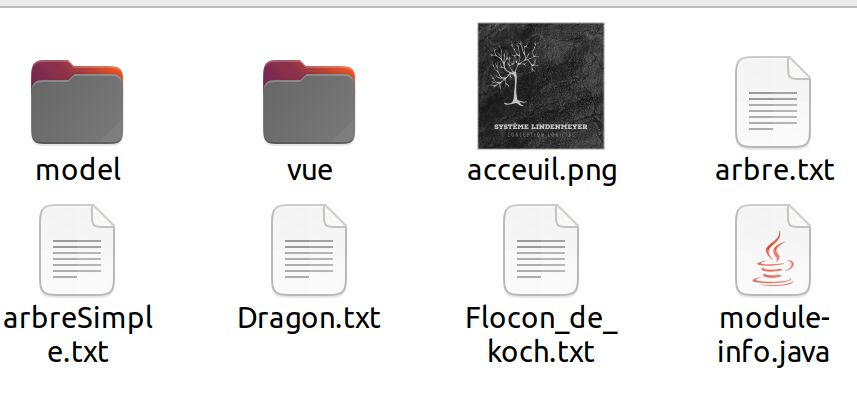
\includegraphics[scale=0.3]{images/fichier.png}
    \caption{Exemple du format des fichiers}
    \end{figure}

    \begin{figure}[h]
    \centering
    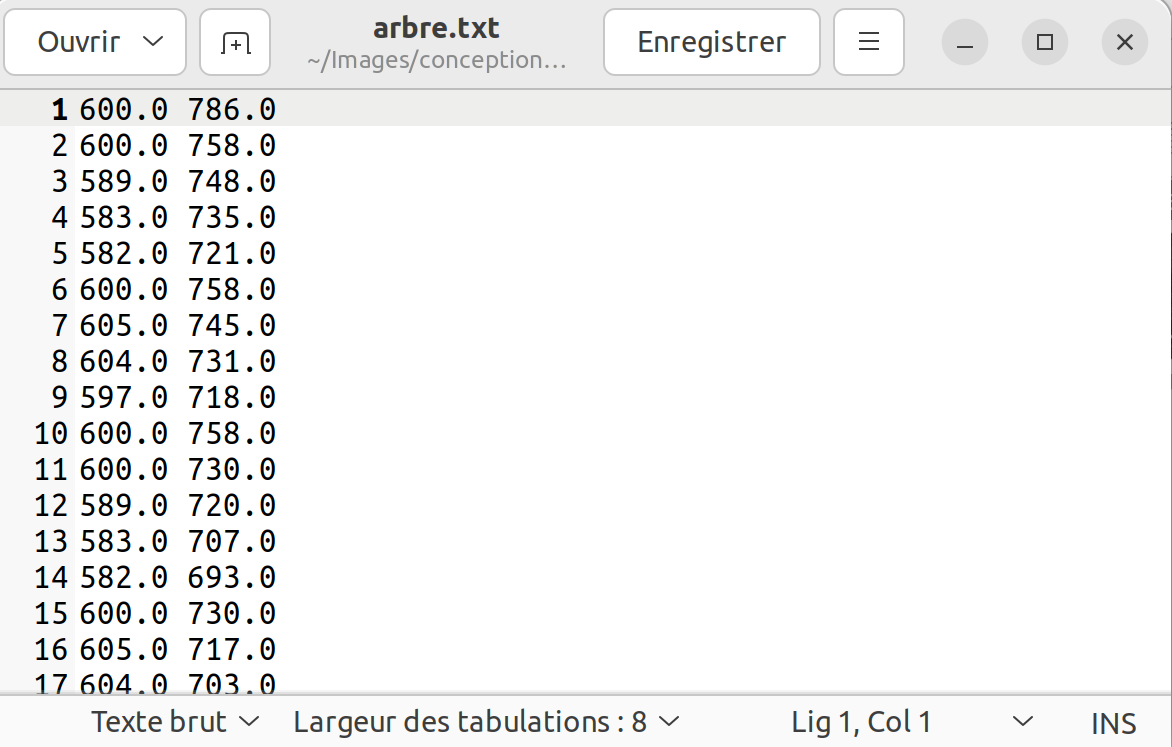
\includegraphics[scale=0.3]{images/contenufichier.png}
    \caption{Exemple contenu du fichier arbre.txt qui réalise le dessin d'un arbre  . }
    \end{figure}

    \newpage
    \end{enumerate}
   
   
  \textbf{Cette partie sera détaillier dans les prochaines sections.}\ref{intro}

   

\subsubsection{Partie 3: Implémentation d'un interpréteur pour une visualisation 3D}

\begin{enumerate}
    \item Extension du moteur de réécriture pour générer des structures tridimensionnelles en utilisant des règles de réécriture spécifiques.En utilisant la fonction "rotation3D(....)"
    \item Explication du processus de transformation des symboles générés en un modèle 3D en utilisant des primitives géométriques comme des cylindres, des sphères, etc.
    \item Utilisation d'une bibliothèque de rendu 3D pour afficher et manipuler les modèles 3D générés à partir du L-système.Avec la bibliothéque \textbf{joagl}.
\end{enumerate}
    
\subsubsection{Partie 4: Extension du langage et des interpréteurs pour des systèmes stochastiques et/ou contextuels}

  \begin{enumerate}
      \item Description des L-systèmes stochastiques\ref{sto}, où les règles de réécriture ont une probabilité d'être appliquées, et des L-systèmes contextuels\ref{con}, où les règlessont conditionnelles et dépendent du contexte environnant.

    \item Extension du langage et du parser pour prendre en compte les règles de réécriture stochastiques et contextuelles, et adaptation du moteur de réécriture en conséquence.
    \item Implémentation d'un moteur de réécriture stochastique qui applique les règles de réécriture avec une probabilité donnée pour générer des structures végétales avec une variation aléatoire.
    \item Implémentation d'un moteur de réécriture contextuel qui prend en compte le contexte des symboles adjacents pour appliquer les règles de réécriture, permettant ainsi de générer des structures végétales avec des formes plus réalistes et complexes en fonction de l'environnement.
  \end{enumerate}  

\subsubsection{Partie 5: Ajout de fonctionnalités avancées}

\begin{enumerate}
    \item  Ajout de fonctionnalités avancées telles que la gestion des paramètres, des variables, des itérations et des règles conditionnelles pour permettre une plus grande flexibilité dans la génération de structures végétales.gérer par des \textbf{try and catch} dans le package "Vue.FenetreLSysteme"
    \item Extension du langage et du parser pour prendre en charge ces fonctionnalités avancées et adaptation des moteurs de réécriture en conséquence.
    \item  Implémentation d'un système de gestion des paramètres pour permettre la modification dynamique des valeurs des paramètres du L-système pendant la génération des structures végétales.
    \item Mise en œuvre d'un système d'itérations pour permettre la répétition d'un ensemble de règles de réécriture un certain nombre de fois, ce qui permet de générer des structures végétales avec des niveaux de détail différents.
    \item Implémentation de règles conditionnelles pour permettre l'application de règles de réécriture en fonction de conditions spécifiques, offrant ainsi plus de contrôle sur la génération des structures végétales en fonction de certains critères.
\end{enumerate}
   
    
   
    
  

    
   

\subsection{Organisation et répartition des tâches}


La répartition des tâches pour le projet de conception s'est organisée en deux binômes, l'un travaillant sur la partie console du projet et l'autre sur la partie interface utilisateur. Cependant,je tiens a vous signaler que le nombre de commits sur SVN peut sembler faible pour chaque membre du groupe, car la plupart du temps, le travail a été réalisé en collaboration et en binôme, ce qui implique que les contributions individuelles ne sont pas nécessairement reflétées uniquement par le nombre de commits.